% Don't always start chapter on new page. (http://tex.stackexchange.com/questions/24066/)
\makeatletter
\patchcmd{\chapter}{\if@openright\cleardoublepage\else\clearpage\fi}{\vspace{1in}}{}{}
\makeatother

\nonfrenchspacing

\chapter{Introduction}
\label{sec:intro}
\textit{DidFail} (Droid Intent Data Flow Analysis for Information Leakage) is
a static analyzer, developed by the CERT Division of the Software Engineering Institute (SEI) at Carnegie Mellon University. DidFail detects possible flows of sensitive
information in sets of Android apps. 
This technical report describes enhancements recently made to the analyzer
itself, a new testing framework, newly developed test apps, and test results. 

The permission system is an important feature of Android security. By placing adjustable limitations on what resources applications can use, Android allows users a large degree of control over how much trust should be given to specific applications. This system allows untrusted applications to coexist in an environment with sensitive information, such as the user's location, contacts, and other personal details.

One of the core assumptions of the Android permission system is that an application that lacks permission to access a resource cannot obtain access to that resource. This assumption is enforced with code that checks that an application has permission for a resource when it requests it from the system. Once the application has access to the resource, however, it can use that resource as it sees fit. This ability to freely use the resource can include sharing private information with other applications or executing actions on behalf of other applications. Indeed, while the Android permission system is well suited for controlling access for applications in isolation, it can fail to protect resources on the device.

Consider the case where a user installs an application for recording audio notes. Because the user is recording sensitive information, he or she verifies that the application has no network access. The same user then installs a weather application that uses the internet but has access to no sensitive content. Considering the applications in isolation, the user has made sensible decisions; the application that has internet access does not have access to sensitive information and vice versa. If, however, these applications can communicate (either intentionally or unintentionally), then the user's information may be at risk. If the audio recording application can send messages to the weather app that are then sent over the internet, an outside attacker could gain access to audio recorded by the device.

Considering the Android permission system alone is insufficient for reasoning about scenarios where information flow between applications circumvents intended permission limitations. \emph{DidFail} is a tool for detecting such flows~\cite{didfail}. DidFail statically analyzes sets of Android application packages (APKs) to detect cases where sensitive information may be leaked from one application to another. While DidFail is a useful tool, it previously fell short in several scenarios. In its previous release, DidFail tracked flows between Activities only by intents. Other types of dataflows, such as those through static fields or between an Activity and a BroadcastReceiver, were missed. With the work detailed in this report, we expanded DidFail's capabilities to work with more applications and handle more types of flows.\footnote{Some flow types are yet to be implemented.} In sections \ref{chap:services} through \ref{chap:infrastructure}, we detail four improved DidFail features.

The main DidFail webpage is \url{http://www.cert.org/secure-coding/tools/didfail.cfm}.  The version of DidFail and the test apps described in this report are also directly available on the Carnegie Mellon University website: 
\\ \url{https://www.cs.cmu.edu/~wklieber/didfail/install-latest.html}.

\chapter{DidFail}

DidFail is a static analysis tool for Android applications that detects possible information flows between applications. DidFail works using two phases.

In Phase 1 (Figure~\ref{fig:overview_phase1}), each APK is fed into the \emph{APK Transformer}, a tool that annotates intent-related function calls with information that uniquely identifies individual cases where intents are used in the application. Once completed, the transformed APK is passed to two other tools: FlowDroid~\cite{flowdroid} and Epicc~\cite{epicc}.

\begin{figure}[h]
	\centering
	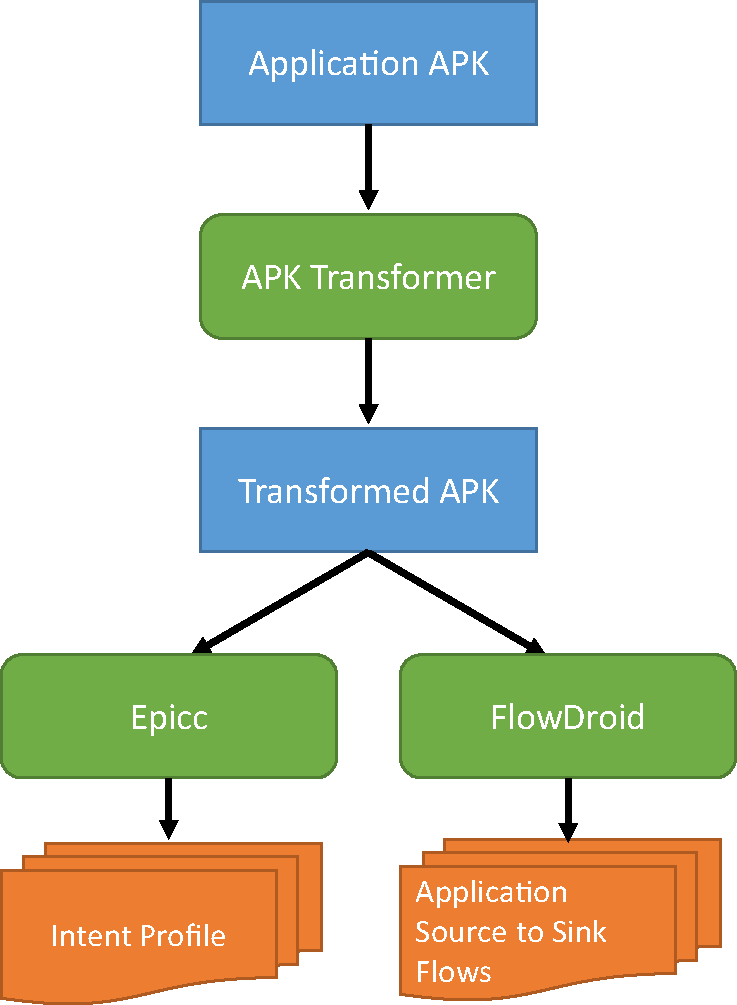
\includegraphics[width=0.35\textwidth]{didfail1.pdf}
	\caption{Overview of DidFail Phase 1}
	\label{fig:overview_phase1}
\end{figure}

The FlowDroid tool performs static taint tracking in Android applications. Given a set of method signatures that correspond to taint sources and sinks, FlowDroid conservatively propagates taint from sources in the application, reporting all flows from sensitive sources to sinks. Sources include function calls that access sensitive information in Android, such as \texttt{getLatitude()} or \texttt{getSimSerialNumber()}. Sinks include function calls that exfiltrate information, such as \texttt{Log.d} and \texttt{FileOutputStream.write}. In addition, reads from received intents are treated as sources, and writes to intents are treated as sinks. Output from FlowDroid might identify, for example, that an application reads contact information from some source, then sends it as part of an intent, or that an application reads information from an intent, then sends it as a Short Message Service (SMS) message.

Epicc~\cite{epicc} performs static analysis to map out inter-component communication within an Android application. While this analysis is mainly used to understand how parts of a single application work together, it can also discover what portions of the application are externally accessible via either explicit or implicit intents. While FlowDroid is useful for understanding flows within an application, Epicc reveals the interfaces that can be used for an application to communicate with other applications.

Phase 1 of DidFail can be performed on one application at a time and, once completed, does not need to be run again.

Phase 2 of FlowDroid combines the Phase 1 output of multiple applications to determine how specific applications in a set can interact. Consider our example from Section~\ref{sec:intro} of the audio and weather applications. If these applications colluded via an intent, then in Phase 1, DidFail would discover that the audio app obtains audio information (a taint source) and the information flows to an intent sent to an application with a specific name.

Similarly, Phase 1 would reveal that the weather app handles intents, reads information from the intent, and then sends it over the internet. 

In Phase 2, DidFail combines the information about these two applications. DidFail analyzes dataflows between apps that can occur through intents, eventually discovering and reporting that sensitive audio information is sent over the internet.

Cases like this one are where DidFail shines. 
Unfortunately, the tool is still limited in the types of flows it can analyze. In our work, we enhanced DidFail to handle more applications and more types of flows.
\newpage
\phantomsection
\chapter{Flows Involving Services} \label{chap:services}
A Service is an application component that is meant to run without direct user interaction (e.g., provide some functionality while the app is not in the foreground). A Service can be instantiated by passing an intent corresponding to a Service's intent filter, or the name of the class instance, and making a call to the \texttt{startService} method. We added new functionality to DidFail to handle some dataflows involving Services.  

\section{General Modifications}
The following sections describe the general modifications we made to the DidFail tool.
\subsection{Recognizing New Intent Sinks}
DidFail's \emph{APK Transformer} identifies intent sinks in an Android app by matching method signatures in the app with known intent sink method signatures. If the signatures match, an intent ID is generated for the intent sink method. Method signatures for the non-Activity intent sinks were added to track intent sinks for BroadcastReceivers and Services. Similarly, FlowDroid had to be modified slightly to recognize the new intent sinks. 

\subsection{Matching Flows by Component Types}
DidFail initially handled only flows involving activities. Extending DidFail to also support BroadcastReceiver and Service components required a slight modification to how the sources and sinks were matched. Certain methods indicate the type of a receiving component and need to be accounted for when matching receiving components and sending components $(e.g.,\  \emph{startService} \rightarrow service, \emph{startActivity} \rightarrow activity).$ By recording the sink component type, we enabled the matching process to create appropriate flows.

\section{Initial Test Results}
Using two apps we created, we tested the analyzer on a single app set. \emph{SendApp}'s main Activity component obtains location information by calling \texttt{getLocation()} and stores the information in an intent set with a custom action string matching \emph{SendAppService}'s intent filter.

As illustrated in Figure~\ref{fig:servicetest1}, the intent is passed to \texttt{startService}, received by \emph{SendApp}'s Service component, and similarly sent to the \emph{ReceiveAppService} component. \emph{ReceiveAppService} passes the tainted information to \emph{ReceiveApp}'s Activity component by calling \texttt{startActivity}.

\begin{figure}[h]
	\centering
%	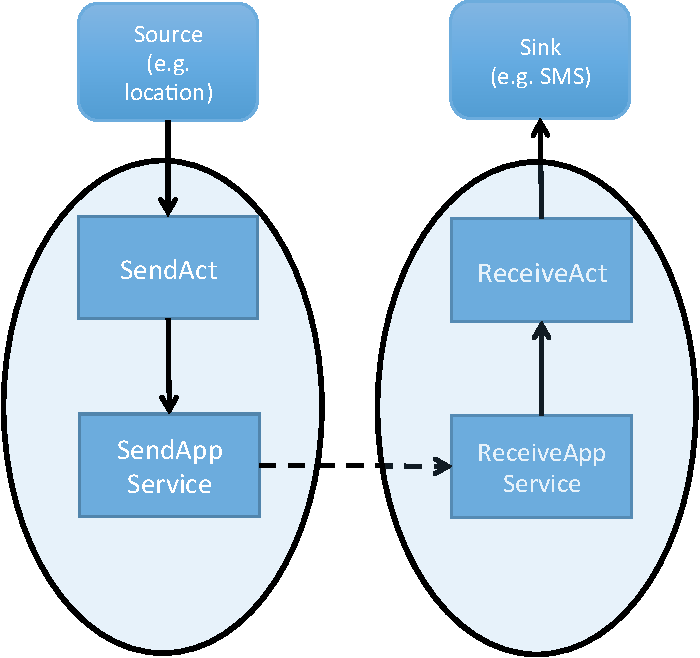
\includegraphics[width=0.35\textwidth]{serviceapp.pdf}
	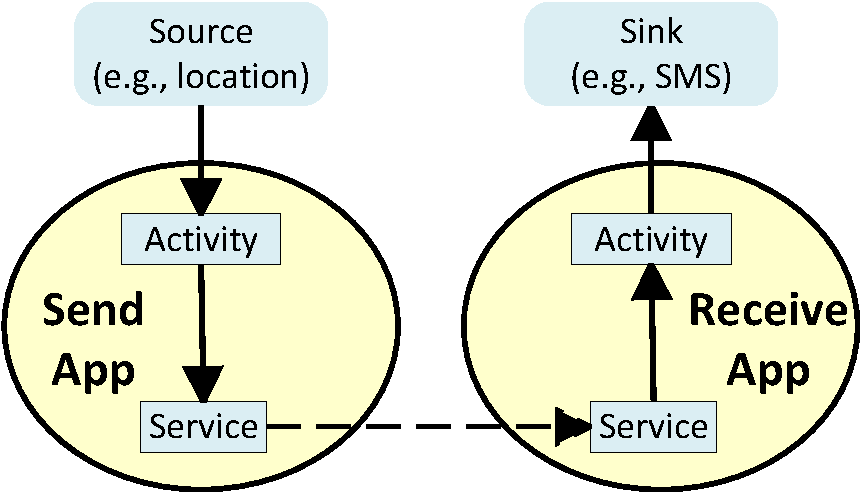
\includegraphics[width=0.50\textwidth]{serviceapps_v2_crop.pdf}
	\caption{Initial App Set for Service Components}
	\label{fig:servicetest1}
\end{figure}

Phase 1 and Phase 2 analysis results were as we expected, tracing the tainted location information through the Activity and Service components as well as identifying the sources and sinks. We also ran a preliminary test of 100 APKs for Phase 1 using the extended APK Transformer, Epicc, and FlowDroid. We observed that intent sinks, such as \texttt{startService} and \texttt{bindService}, were identified. Further testing still needs to be done to verify that the modifications improve Phase 2 results.

\newpage
\phantomsection
\chapter{Flows Involving BroadcastReceivers} \label{chap:broadcast_receivers}
Previous versions of DidFail failed to detect dataflows that involve broadcast intents. Broadcast intents are received in a particular way; the app contains a class that extends the class \texttt{android.content.BroadcastReceiver}, which implements the \texttt{onReceive} method. An application can declare the broadcasts it wishes to receive statically in the manifest or dynamically with the \texttt{registerReceiver()} method. There are different types of broadcasts: normal broadcasts with unordered receivers, ordered broadcasts, and sticky broadcasts that remain active after the initial broadcast distribution is completed.

An app can unregister a dynamically registered receiver (and thereby stop it from receiving broadcasts) by calling the \texttt{Context.unregisterReceiver()} method.  DidFail does not consider calls to \texttt{unregisterReceiver()}; if it can be proven that a receiver cannot be live when a tainted broadcast is sent, then DidFail produces a false alarm.

We made three modifications to allow DidFail to analyze dataflows that include broadcast intents. As mentioned in Section 4.6, a manual adjustment is necessary to handle dynamically registered receivers, and we do not yet analyze for the dataflow of sticky broadcasts and ordered broadcasts. We enhanced the Epicc parser to extract information about broadcast intents, modified FlowDroid to mark broadcast-related functions as sources or sinks, and extended Phase 2 to consume the new output resulting from the previous modifications.

\section{Parsing Epicc Output for BroadcastReceivers}
Dynamically registered receivers do not appear in the manifest, but they do appear in the output of Epicc.  An entry starts with the line ``\texttt{Type:\ android.content.BroadcastReceiver}."  Potential filter properties are given as a list (for example, the Actions field in Figure~\ref{fig:bcast_epicc_output}).

\begin{figure}[!h]
\begin{framed}
\verbatiminput{epicc_br_out.txt}
\caption{Example Epicc Output for a BroadcastReceiver}
\label{fig:bcast_epicc_output}
\end{framed}
\end{figure}

We added a separate parser function named \texttt{parse\_bcast} to address this issue. It is used by DidFail in addition to the previously existing parser function named \texttt{epicc\_parser}.

\section{Marking Broadcast Intents as a Sink/Source in FlowDroid}
Function signatures related to transmitting and receiving broadcast intents were added to the APK Transformer and FlowDroid so that they were recognized as sources or sinks. Table~\ref{fnc_bcast} shows the related functions.
\begin{table}[!h]
\renewcommand{\arraystretch}{1.3}
\caption{Functions Related to Broadcasting Intents}
\label{fnc_bcast}
\centering
\rule{0.55\textwidth}{0.75pt}
\\
\tt
\begin{tabular}{l}
%\hline
onReceive \\
sendBroadcast \\
sendBroadcastAsUser \\
sendOrderedBroadcast \\
sendOrderedBroadcastAsUser \\
sendStickyBroadcast \\
sendStickyBroadcastAsUser \\
sendStickyOrderedBroadcast \\
sendStickyOrderedBroadcastAsUser \\
%\hline
\end{tabular}
\\
\rule{0.55\textwidth}{0.75pt}
\end{table}

\section{Trace Broadcast Flows in Phase 2}
The \texttt{taintflows.py} program (responsible for executing Phase 2 of DidFail) was extended to parse the additional sinks and sources introduced in the previous sections and to match broadcast intent filters. The logic is the same as with non-broadcast intents.

\section{Test Applications}
We wrote four apps to test this new feature:

\begin{itemize}
\item{} \emph{BroadcastTx} has the READ\_PHONE\_STATE permission and sends the device ID via a broadcast intent with an action filter. See Figure~\ref{fig:broadcastleak} for the code that leaks the device ID.

\item{} \emph{BroadcastRx\_Static} has the SEND\_SMS permission and receives broadcast intents via a statically declared receiver with the same action filter as declared in the manifest file.  See Figure~\ref{fig:broadcastmanifest} for the manifest, and Figure~\ref{fig:broadcaststaticrecvr} for the receiver class.

\item{} \emph{BroadcastRx\_Dyn} has the ACCESS\_FINE\_LOCATION permission and receives a broadcast intent via a dynamically registered receiver with the same filter.  See Figure~\ref{fig:broadcastregister} for the receiver registration, and see Figure~\ref{fig:broadcastdynrecvr} for the receiver class. 

\item{} \emph{KludgeBroadcastRxDyn} is the same as \emph{BroadcastRx\_Dyn}, except it has a filter declaration in the manifest (see Figure~\ref{fig:broadcastDynManifestKludge}) as well as a standard dynamic registration of the BroadcastReceiver in the component’s Java code. 
\end{itemize} 


\begin{figure}[!h]
\begin{framed}
\lstinputlisting[language=Java]{java/broadcasttx.java}
\caption{Transmitter Code Leaking Device ID Through a Broadcast Intent}
\label{fig:broadcastleak}
\end{framed}
\end{figure}

\begin{figure}[!h]
\begin{framed}
\lstinputlisting[language=XML]{broadcaststatic.xml}
\caption{Statically Declared BroadcastReceiver in a Manifest File}
\label{fig:broadcastmanifest}
\end{framed}
\end{figure}

\begin{figure}[!h]
\begin{framed}
\lstinputlisting[language=Java]{java/broadcastonreceive.java}
\caption{Code for a BroadcastReceiver that Sends Text Messages}
\label{fig:broadcaststaticrecvr}
\end{framed}
\end{figure}

\begin{figure}[!h]
\begin{framed}
\lstinputlisting[language=Java]{java/broadcastDynManifestKludge.java}
\caption{Manifest Code of \emph{KludgeBroadcastRxDyn}, with Manually Added Filter for Dynamically Registered BroadcastReceiver}
\label{fig:broadcastDynManifestKludge}
\end{framed}
\end{figure}

\begin{figure}[!h]
\begin{framed}
\lstinputlisting[language=Java]{java/broadcastdyn.java}
\caption{Registering a BroadcastReceiver Dynamically}
\label{fig:broadcastregister}
\end{framed}
\end{figure}

\
\begin{figure}[!h]
\begin{framed}
\lstinputlisting[language=Java]{java/broadcastdynrcvr.java}
\caption{Code for a BroadcastReceiver that Writes to a File}
\label{fig:broadcastdynrecvr}
\end{framed}
\end{figure}

\section{Results}

Our modified FlowDroid identified the expected flows from sources to sinks in three of the four toy applications: \textit{BroadcastTx}, \textit{BroadcastRx Static}, and \textit{KludgeBroadcastRxDyn}. For these apps, it identified the leakage of the device ID through a broadcast intent in Figure~\ref{fig:broadcastleak} as a tainted source. The BroadcastReceivers in Figure~\ref{fig:broadcaststaticrecvr} and Figure~\ref{fig:broadcastdynrecvr} were identified as sinks.

Phase 2 analysis correctly identified two inter-application flows: (1) from the transmitter to the statically registered BroadcastReceiver and (2) from the transmitter to the dynamically registered BroadcastReceiver.

DidFail did not detect the dataflows from sources to sinks in the other app, \textit{BroadcastRx\_Dyn}, for reasons described in Section 4.6.

Because FlowDroid was unable to statically detect flows in \textit{BroadcastRx\_Dyn}, we tested this app on a physical phone, alongside \textit{BroadcastTx}. Figure~\ref{fig:logcat-BcastDyn} shows the log messages (from \ttt{adb logcat}) when running \textit{BroadcastTx} and \textit{BroadcastRx\_Dyn}.

\begin{figure}[!h]
\begin{framed}
\begin{alltt}
D/BcastTx (28361): OnClick
D/BcastTx (28361): DeviceID: 35███████████03
D/BcastTx (28361): Intent has been sent.
D/BcastRxDyn(28399): 35███████████03
\end{alltt}
\caption[Output of \ttt{adb logcat}]{Output of \ttt{adb logcat} (The Device ID Has Been Partially Redacted.)}
\label{fig:logcat-BcastDyn}
\end{framed}
\end{figure}

\section{Dynamically Registered BroadcastReceivers}
Currently, for a dynamically registered BroadcastReceiver to be handled by DidFail, a dummy static declaration of the BroadcastReceiver must be added to the manifest file so that FlowDroid can appropriately analyze it. This dummy declaration can be added after analysis of the code shows a BroadcastReceiver is dynamically registered, as successfully demonstrated in the test app \textit{KludgeBroadcastRxDyn}.\footnote{This and the other test apps we developed for this project are available for free download at http://www.cs.cmu.edu/~wklieber/didfail/test-apps-dec2014/}

Some problems with analyzing dynamically registered BroadcastReceivers have been fixed in the latest version of FlowDroid’s development branch. The develop branch of the standard FlowDroid distribution\footnote{https://github.com/secure-software-engineering/soot-infoflow-android} has newly added handling of some dataflows involving dynamically declared BroadcastReceivers. Their DroidBench\footnote{https://github.com/secure-software-engineering/DroidBench/tree/develop} test app distribution now includes two apps (\textit{BroadcastReceiverLifecycle2} and \textit{BroadcastTaintAndLeak1}), which have dynamically declared BroadcastReceivers with taint flows that FlowDroid detects, and it detects taint flow in our test app \textit{KludgeBroadcastRxDyn}. However, at the time of this writing, the taint flow in our test app \textit{BroadcastRx\_Dyn} is not detected by FlowDroid.

\section{Future Work}
We plan to modify DidFail to handle dynamically declared BroadcastReceivers in a fully automated way by integrating it with a recent version of FlowDroid and working to fix remaining un-analyzed taint flows. We plan to investigate modifying FlowDroid to analyze the flows, or alternatively, modifying the APK Transformer to automatically add this dummy declaration into the app’s manifest file. We also plan to add analysis specific to ordered and sticky broadcasts.


\newpage
\phantomsection
\chapter{Flows Involving Static Fields} \label{chap:static_fields}

There are many ways that Android apps could communicate. The most direct way is for applications to send and receive intents, which are specifically designed for inter-application communication. Other, more subtle communication mechanisms can also be used to share information between applications, including cooperative use of shared state, or covert channels such as power usage and timing. DidFail needs to understand as many communication channels as possible, to determine how applications share permissions.

\section{The Issue with Static Fields}

While DidFail does not detect many of these communication channels, support was successfully added for detecting some flows through \emph{static shared fields}. A static field in Java (denoted by using the \texttt{static} keyword) shares its value among all instances of the class. The declaration of static fields establishes state at the class level rather than at the instance level.

Static fields present an interesting challenge when trying to detect inter-application flows on Android. Consider a hypothetical application, \emph{AppChat}, that receives intents, appends the contents of received intents to a static String \texttt{holdover}, and then returns the contents of \texttt{holdover} to the application that originally issued the intent. This \emph{AppChat} application allows two applications (\emph{A} and \emph{B}) to communicate with each other via proxy. \emph{A} can send a message to \emph{AppChat}; that message is saved in the static field \texttt{chatlog}. When \emph{B} sends a message to \emph{AppChat}, it will receive back the message sent to \emph{AppChat} by \emph{A}. Consequently, in the application set containing \emph{A}, \emph{B}, and \emph{AppChat}, there exist six potential inter-application flows: \emph{A$\rightarrow$AppChat}, \emph{AppChat$\rightarrow$A}, \emph{B$\rightarrow$AppChat}, \emph{AppChat$\rightarrow$B}, \emph{A$\rightarrow$B}, and \emph{B$\rightarrow$A}.

\begin{figure}
\begin{framed}
\lstinputlisting[language=Java]{java/appchat.java}
\caption{Simple Static Field Example (Simplified Version of AppChat Code)}
\label{fig:appchat}
\end{framed}
\end{figure}

Unfortunately, DidFail originally failed to detect some of these potential flows, due to its use of the FlowDroid tool~\cite{flowdroid}. FlowDroid statically detects potential flows from labeled source and sink functions in an APK. In this case, \texttt{getIntent} is considered a source, while \texttt{setResult} is considered a sink. Consequently, FlowDroid reports a single flow from \texttt{getIntent} to \texttt{setResult}. Notably, this result is the same as if the static field \texttt{holdover} had not been used at all (that is, the received message is echoed back as the reply). Indeed, while FlowDroid does track through static fields, it does not indicate their presence in the results. As a result, the second phase of DidFail is unaware of the presence of any static fields in an application.

Given only the flow from \texttt{getIntent} to \texttt{setResult}, DidFail understood that the \emph{AppChat} application accepts input from an application and then replies to that application based on that input. As a result, DidFail reported the following flows: $I_A\rightarrow R(I_A)$ and $I_B\rightarrow R(I_B)$. These flows account for four of the six of the flows we described above (\emph{A$\rightarrow$AppChat}, \emph{AppChat$\rightarrow$A}, \emph{B$\rightarrow$AppChat}, \emph{AppChat$\rightarrow$B}). Crucially missing, however, was the flow between applications \emph{A} and \emph{B}, which can communicate via the static field \texttt{holdover}. 

\section{Adding Support for Static Field Flows}

For DidFail to analyze flows involving static fields, FlowDroid needed to be modified to report about how static fields are used in an application. Given that static fields provide a persistent state that can be both read from and written to, it makes sense to treat static fields as both a source \emph{and} a sink. In other words, if sensitive information flows from a source to a static field, we should report the flow, and if content flows from a static field to a sink, we should report that flow as well.

There were a number of key challenges we encountered while trying to add this feature to FlowDroid. First and foremost, FlowDroid handles only sources and sinks that occur as function calls. Consequently, while it is easy to mark a function as a new taint source, there is no support for adding more general types of sources, such as those associated with a specific variable. This limitation meant that we needed to modify the actual code associated with FlowDroid's taint analysis to achieve our goals.

At a high level, FlowDroid discovers flows in an application using the following steps:
\begin{enumerate}
\item Load source code of the application, convert the code to Jimple~\cite{soot}, and construct an \emph{exploded supergraph} that models interprocedural interactions. Note that a node is a statement in Jimple, and an edge is directed, pointing from a node $A$ to $B$, if $B$ can succeed $A$ in some possible program execution. Each node also has a taint status T.
\item Scan through the graph and add an edge ($\emptyset$, $N$) for every $N$ that contains a source to a worklist $W$.
\item While $W$ is non-empty, pop edge $(N_1, N_2)$ from $W$:
\begin{enumerate}
\item Given the current taint status on $N_1$, run the \emph{flow function} on $(N_1, N_2)$ to produce the current taint status for $N_2$.
\item If the taint status of $N_2$ changed, for every child of $N_2$, $N_3$, add edge $(N_2, N_3)$ to the worklist $W$.
\end{enumerate}
\item Use the per-statement taint information to compute the source-to-sink flows through the application.
\end{enumerate}

The majority of this algorithm is based on the general IFDS Framework for dataflow analysis~\cite{ifds}. The key component of FlowDroid's instantiation are the \emph{flow functions} used to propagate taint information across edges. These flow functions, one of which is selected based on the type of statement in question, dictate when taint information is created, propagated, and destroyed. Consider an assignment statement $x = y$. If $y$ is tainted, then we should mark $x$ as tainted, and if $y$ is not tainted, then we do not mark $x$ as tainted. 

In the original FlowDroid, because all taint sources and sinks are function calls, an assignment of the form $x = y$ can only propagate taint, not create or destroy it. To support static fields, however, this approach must be changed. We modified the flow function for assignment statements of the form $x = y$ to instead have the following logic:

\begin{itemize}
\item If $y$ is a static field, mark $x$ with taint $T_y$, where $T_y$ is taint originating from static field $y$.
\item If $x$ is a static field and $y$ is tainted with taint $T$, add a $T\rightarrow x$ to the list of sink results.
\item Otherwise, the taint of $x$ is set to the taint of $y$.
\end{itemize}

In addition, we altered the original code that seeds the IFDS algorithm with initial edges to also add edges for assignment statements involving reads from static fields. This modification works quite well for basic examples. FlowDroid now correctly reports the flows $getIntent\rightarrow holdover$, $holdover\rightarrow setResult$; and $getIntent\rightarrow setResult$ from the Figure~\ref{fig:appchat} example. With the static field information now recorded as extra information flows, judgments can now be made about inter-application flows through static fields. (See Section~\ref{sec:staticphase2}.)

\section{Harder Static Field Flows}

\begin{figure}
\begin{framed}
\begin{center}
\begin{minipage}{0.85\textwidth}
\lstinputlisting[language=Java, numbers=left]{java/aliased.java}
\end{minipage}
\end{center}
\caption{Static Fields with Aliasing}
\label{fig:aliased}
\end{framed}
\end{figure}

Unfortunately, this simple solution does not work in a non-trivial case. Consider the situation where a static variable has been \emph{aliased}, as in Figure~\ref{fig:aliased}. In this case, when we run the flow function on the line $\mathit{b2}.x = source()$, we should treat $\mathit{b2}.x$ as a sink because it is a static field. It is not obvious that term $\mathit{b2}.x$ is a static field, however. It is only the fact that $\mathit{b2}.x$ comes after the line $\mathit{b2} = b$ that causes it to be a static field. What this reveals is that, in the general case, \emph{context is necessary} for identifying static fields. If $\mathit{b2}.x$ occurred after $\mathit{b2} = new Box()$, then $\mathit{b2}.x$ would not be considered to be a sink on Line 8.

Naturally, whether a given term $x.y.z... = t$ is a write to a static field is an undecidable property. We can, however, obtain a conservative guess of which fields are static by creating an additional FlowDroid pass that occurs before the main taint analysis. This pass, which uses the same type of taint analysis, marks all static variables as sources and then propagates taint forward. For the code in Figure~\ref{fig:aliased}, $b$ would be tainted on Line 7, which would cause $\mathit{b2}$ to be tainted. Because $\mathit{b2}$ is tainted, $\mathit{b2}.x$ is also tainted. Once we finish with this initial pass, we record the results of what is tainted in a set.

With this initial pass completed, we now have enough information to solve our aliasing problem. We no longer need to guess whether $\mathit{b2}.x$ is a static field; we can simply check whether it is in the set of statements marked as tainted in the first pass. With this modification, our flow function for assignment $y = x$ now becomes the following:

\begin{itemize}
\item If $y$ is a static field, mark $x$ with taint $T_x$, where $T_x$ is taint originating from static field $x$.
\item If $x$ is a static field \textbf{OR $x$ is in the set of tainted statements from Pass 1}, and $y$ is tainted with taint $T$, add a $T\rightarrow x$ to the list of sink results.
\item Otherwise, the taint of $x$ is set to the taint of $y$.
\end{itemize}

This reuse of FlowDroid's taint analysis to find static fields turns out to be a pleasant and concise solution. In contrast, our initial attempts at a solution in one pass that involved backtracking were much more complex and did not generalize well.

\section{Phase II Static Field Analysis}
\label{sec:staticphase2}

Phase II still needs to make use of the flows through static fields information produced in Phase I. Recall that in our original example involving applications $A$, $B$, and $AppChat$, DidFail found the flows $I_A\rightarrow R(I_A)$ and $I_B\rightarrow R(I_B)$, where $I_A$ and $I_B$ are intents issued by $A$ and $B$, respectively. 

When we run modified FlowDroid on $AppChat$, we obtain the flows $getIntent\rightarrow holdover$, $holdover\rightarrow setResult$, and $getIntent\rightarrow setResult$, as stated earlier. Because $holdover$ is a static field that could persist across the handling of multiple intents, \emph{every application} that reads from $holdover$ is tainted by \emph{every application} that writes to that static field. This approach effectively amounts to taking the Cartesian product of all reads and writes to the field. We find that application $A$ and $B$ both write to and read from $holdover$, so taking the Cartesian product, we get $(A, A), (A, B), (B, A),$ and $(B, B)$. This result means that in addition to the flow where $A$ and $B$ interact with $AppChat$ in isolation, we must now consider the case where input from $A$ flows to $B$ and vice versa.

These additional flows from the Cartesian product calculation are added to the set of flows after DidFail generates the Phase II flow equations. (Generating the Phase II flow equations is described in detail in Section 3.3 of \cite{didfail}). 

\section{Results} \label{sec:static-results}
Our enhanced DidFail identified the expected flows from sources to sinks in a set of three toy apps we developed, which provided the taint flow described in sections 5.1 and 5.4: \emph{AppChat}, \emph{SendSMS2}, and \emph{LogWrite}. \emph{SendSMS2} calls source method \texttt{getLine1Number()},  which gets the MSISDN for a GSM phone.  \emph{SendSMS2} sends data it receives from \emph{AppChat} into an SMS-sending sink call. \emph{LogWrite} calls source method \texttt{getLastKnownLocation(java.lang.String)} and sends data it receives from \emph{AppChat} into a sink method call to \texttt{Log.w}. DidFail finds that both sources can reach both sinks via  data flows that involve a static field in \emph{AppChat}. 

Figure~\ref{fig:staticAnalysisProblem} shows an example static field setup where FlowDroid fails to identify any flow through the static field, and so our modifications also fail to trace taint through it.  The taint flow analysis fails to detect flows, for flows involving fields of static classes that another class gets and sets.

\begin{figure}
\begin{framed}
\begin{center}
\begin{minipage}{0.85\textwidth}
\lstinputlisting[language=Java, numbers=left]{java/staticFieldProb.java}
\end{minipage}
\end{center}
\caption{Field of Static Class; Other Class Gets and Sets Field}
\label{fig:staticAnalysisProblem}
\end{framed}
\end{figure}


\section{Drawbacks, Limitations, and Future Work}

Our analysis appeared to work correctly, except for fields of static classes that another class gets and sets, as discussed in \ref{sec:static-results}. We plan to modify FlowDroid to detect those taint flows. While our modifications to support flows through static fields worked quite well in most cases, there are some additional issues with our solution. With two taint passes instead of one, that analysis can take twice as long as the original analysis. 

More critically, the FlowDroid runtime also scales with the number of sources, which means that adding a new source for every static field read could also severely impair performance depending on how frequently static fields are used. To evaluate how important this issue is, we tested 100 APKs that, prior to adding this new feature, were successfully analyzed within the allocated time and memory (using virtual machines with 61 GB and FlowDroid analysis memory allowed to take up to 32 GB). (See Section~\ref{sec:infrastructure}.) Unfortunately, the majority (66 out of 100) timed out or ran out of heap space. Most applications make frequent use of static fields, particularly when invoking libraries such as Google Ads. For many of these applications, an additional taint analysis for every static field read was prohibitively expensive. In the future, we will increase virtual machine memory size to see if it enables successful static field taint analysis of more apps. Virtual machines with 244~GB of memory are available,\footnote{\url{http://aws.amazon.com/ec2/pricing/}} which also have 32 virtual cores. Future work will also develop strategies to reduce the number of reads that get traced through the program. 

As noted earlier, detecting which fields are static is undecidable and our taint-based solution is an overapproximation. Consequently, some reported flows to static fields may not be realizable in practice. The solution is not a \emph{strict} over approximation, however, because there are some cases where FlowDroid itself does not recognize that a flow exists at all. We cannot detect flows that use static fields for legitimate flows missed by FlowDroid. 

Finally, the current implementation does not support static fields involving arrays. This feature should be straightforward to add, however.


\phantomsection
\chapter{Infrastructure Improvements} \label{chap:infrastructure}
\label{sec:infrastructure}
The original DidFail implementation experienced a high failure rate in the Phase 1 analysis.  Recall that Phase 1 analysis is run on each APK separately to find tainted flows in these apps.  This first step of the analysis transforms the input APK, instrumenting the callsite of intent-sending methods with a unique ID.  The transformed APK is then processed by FlowDroid and Epicc.  With this improvement, we sought to increase the success rate of APK processing in Phase 1.

\section{The Problem}
We identified several issues that contributed to a high failure rate in Phase 1.  The APK Transformer and FlowDroid rely on the underlying Soot framework to handle reading and writing APK files. While the APK Transformer itself rarely failed, FlowDroid often choked on the APK produced by the APK Transformer.  Moreover, some APKs encountered no explicit FlowDroid failures, but were not analyzable in a timely fashion (the FlowDroid invocation ran out of time or memory). These issues together resulted in a very low success rate in Phase 1. There were no significant issues encountered with the Epicc tool.  In the time since the original DidFail version was completed in March 2014, a new version of the Soot framework was released. This new version included significantly better facilities for handling APK files, but it was not completely compatible with code written against the older version of Soot. A new version of FlowDroid was also released, which used the new version of Soot.

\section{Porting Phase 1}
Our first step was to port the DidFail changes to the latest versions of Soot and FlowDroid.  This step involved inspecting the modifications to the old FlowDroid branch, moving them to the latest FlowDroid branch, and then testing for correctness.  Moreover, the APK Transformer was changed to use the latest version of Soot, requiring a few source changes and further testing.

\section{Measuring Phase 1 Performance}
The next step was to create an instrumented harness for running the various components of Phase 1.  In particular, we were interested in gathering data about FlowDroid, since in previous test runs many APKs timed out during FlowDroid processing.  A small test harness was developed in Python for running various Phase 1 components (the APK Transformer, Epicc, FlowDroid, etc.) with various parameters and with a specified timeout.  This harness also measured system metrics (e.g., memory usage, CPU usage) while the DidFail analyses were running.  

\section{Initial Testing}
A selection of 90 APKs was chosen randomly from a large set, with the goal of running them through both the old and new versions of DidFail to evaluate the effectiveness of our changes.  A machine was provisioned from Amazon EC2 to run the test because it was difficult to secure time on a machine locally with enough resources.  This machine was equipped with 4 cores and 32 GB of memory.  FlowDroid was allocated 16 GB of memory (through the heap space parameter to the JVM) and a 15-minute timeout.  APKs were processed by the APK Transformer before being sent to FlowDroid.  The graph in Figure~\ref{fig:initial_phase1} summarizes the results of this test.

\begin{figure}[h]
	\centering
	\begin{minipage}{0.85\textwidth}
	\centering
	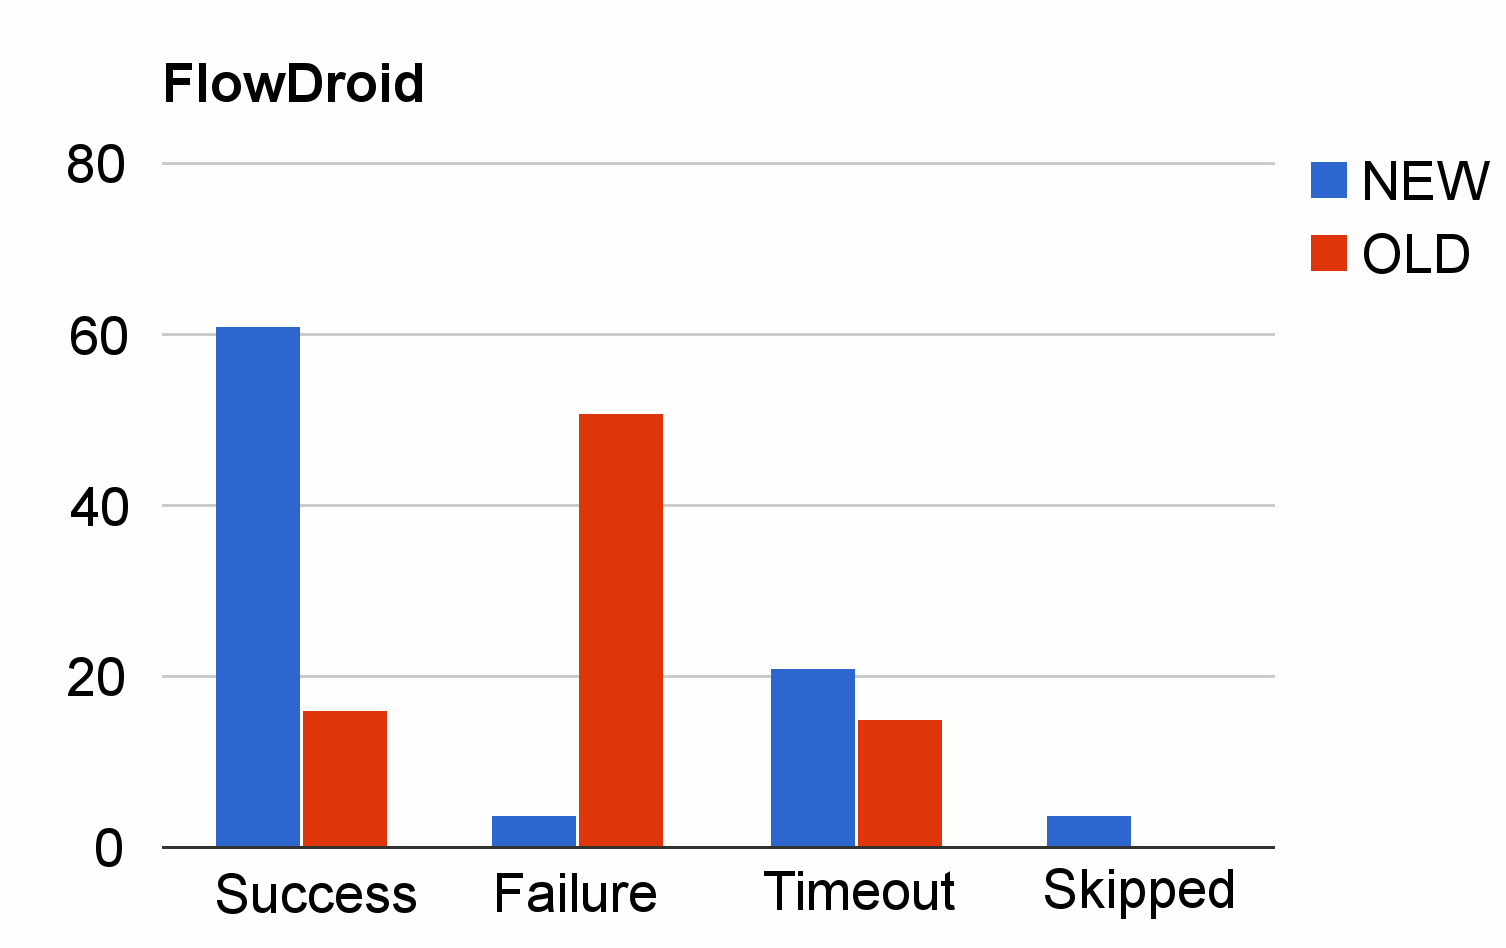
\includegraphics[width=0.66\textwidth]{flowdroid_success2.png}
	\caption[Results of FlowDroid Test Run on 90 Apps, With and Without Modifications]{Results of FlowDroid Test Run, With and Without Modifications}
	\label{fig:initial_phase1}
	\end{minipage}
\end{figure}

The number of APKs successfully processed by FlowDroid roughly tripled from 16 to 61 with very few failures. A few APKs were skipped due to errors in the transformation stage. There were 21 APKs that timed out during FlowDroid analysis\textemdash5 more than timed out in the initial run.  The smaller number of timeouts in the initial run may be explained by the high failure rate; if more APKs hadn't run into runtime exceptions, they may have eventually timed out.  This test run showed that our modifications substantially improved the baseline success rate of Phase 1 analysis.

\section{FlowDroid Performance Tweaks}
Next, we investigated the 21 timeouts in the FlowDroid test.  By reviewing the performance counters, we saw that these analyses consumed all the memory allocated to them (16\,GB) and were unable to make further progress.

The first thing we tried was vertical scaling.  We provisioned a much larger machine and ran FlowDroid again on one of the timed-out APKs.  This run was not productive.  Despite allocating nearly 170GB of memory to the process and disabling timeouts, the analysis reached the same state as before: consuming all allocated memory and making next to no progress.  Figure~\ref{fig:high_phase1} shows memory usage over time (approximately 2 hours) for that analysis attempt.

\begin{figure}[h]
	\centering
	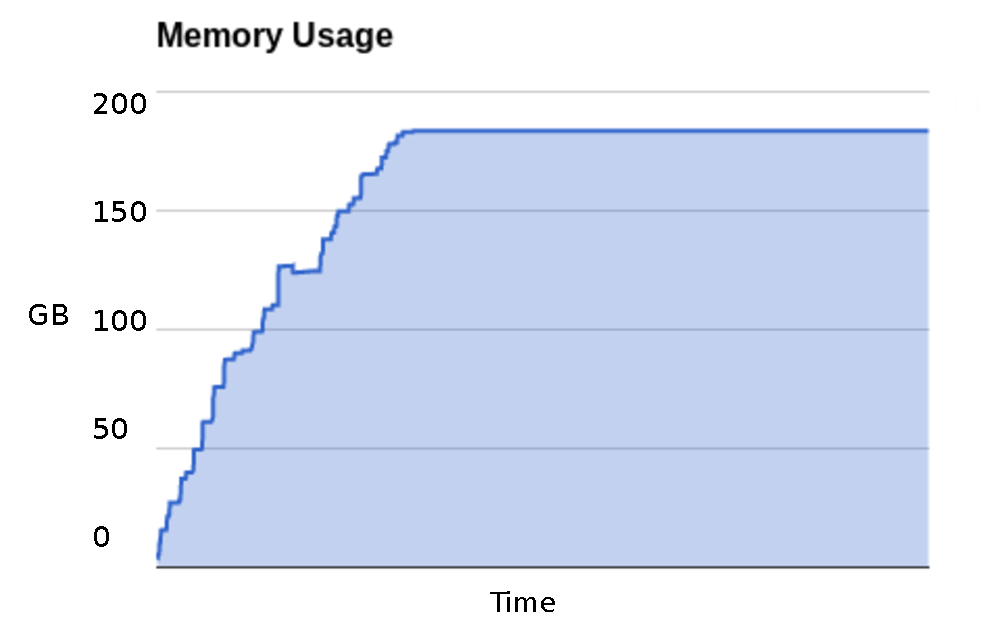
\includegraphics[width=0.50\textwidth]{flowdroid_perf.pdf}
	\caption{Results of the FlowDroid Test Run on a High-Performance Machine}
	\label{fig:high_phase1}
\end{figure}

It was clear that the analysis itself needed to be tuned.  Recall that FlowDroid seeks to construct paths between sources and sinks in an application.  Two fundamental aspects we could tweak were the source/sink identification process and the pathfinding process.  Regarding the former, we could try to reduce the number of sources and sinks by filtering them in some fashion.  Regarding the latter, we could reduce the precision of the pathfinding process.  Of course, this tuning impacts the quality of the analysis.  Filtering the sources/sinks may cause FlowDroid to miss a potentially dangerous flow.  Dumbing down the pathfinding bears this risk as well, and carries the additional risk of introducing false positives. 

Nonetheless, we were interested in determining how much tuning FlowDroid required to process the remaining 21 APKs.  We provisioned the same machine as before (32 GB of memory, 4 cores), and maintained the same timeout (15 minutes).  

Source/sink filtering resulted in 9 out of the 21 APKs getting successfully processed by FlowDroid. Source/sink filtering uses the FlowDroid command-line parameters \ttt{nocallbacks} and \ttt{layoutmode}. The first disables the emulation of Android callbacks (due to button clicks, GPS location changes, etc.), while the second ignores Android GUI components, like input fields, as dataflow sources.

Tuning the pathfinding precision by setting the \ttt{aplength} parameter resulted in six of the twelve remaining APKs succeeding. The \ttt{aplength} parameter accepts an integer and sets the FlowDroid \itc{access path} length. Consider the Java statement \ttt{X.Y.Z = 5}. The left-hand side of the assignment statement has an access path length of 2. Using this parameter, one can configure how deeply FlowDroid will search access paths when tracking taint. With an access path length of 0, all the fields of an object referenced by a variable are conflated, potentially resulting in many false alarms.

Using the \ttt{nopaths} parameter was required for the remaining six APKs to make it through FlowDroid without timing out. The \ttt{nopaths} parameter causes FlowDroid to invest no effort in constructing accurate paths. Rather, it will simply report source/sink pairs. 

Additional options to improve performance are described on the FlowDroid webpage.\footnote{\url{https://github.com/secure-software-engineering/soot-infoflow-android/wiki}} For future testing, we will compare these options in terms of precision versus computation requirements, as we did for the work discussed in this report.


\section{Conclusions and Future Work on Infrastructure Improvements}
We substantially improved the success rate of Phase 1 analysis and investigated the performance of FlowDroid.  We found in many cases that vertical scaling is not a viable solution to FlowDroid timeouts.  Moreover, we found that some APKs will not yield to (timely) FlowDroid analysis without very liberal compromises on path precision.

There are two broad directions for future work in this area.  First, more effort can be invested in Phase 1.  FlowDroid could potentially be made to be more resource efficient.  Also, more configuration options could be added to FlowDroid to allow more granular tuning of the pathfinding process.  Further, the results reported here do not include the modifications made as part of the rest of the project (initial enhancements for analysis of dataflows that traverse shared static fields, Service components, and BroadcastReceiver components).  These additions increase the work required by the Phase 1 analysis, in some cases non-trivially.  At the time of this writing, preliminary results show increased timeouts when FlowDroid is run with these additions using the same hardware configuration.  In summary, building a Phase 1 analysis that accurately finds a wide variety of flows, in a timely fashion, is a difficult problem --- one that requires a variety of compromises. 

Next, Phase 2 analysis needs some attention. There are some interesting questions yet to answer. How does tuning down the precision of Phase 1 affect Phase 2 results?  Now that more APKs can be processed by Phase 1, can we find legitimate, inter-application flows in the wild with Phase 2 analysis?
\newpage
\chapter{Related Work}
Felt et\ al.~\cite{felt2011android} found that about one-third of Android apps (of the 940 they tested) asked for more privileges than they actually used. They also found evidence that one cause of over-privilege is developer confusion, in part due to insufficient Android API documentation. Malicious apps can use permission re-delegation attack methods \cite{felt2011permission} that, when successful, take advantage of a higher-privilege app performing a privileged task for an application without permissions. The Epicc \cite{epicc} tool precisely analyzes inter-app communication in Android.  By looking at intents sent and intent filters (both declared in the manifest file and  dynamically registered in the case of BroadcastReceivers), Epicc can detect vulnerabilities due to app communication, such as activity hijacking. Although it examines vulnerabilities due to intents, the Epicc analysis alone does not trace and identify data flows between sources and sinks. 
TaintDroid~\cite{enck2010taintdroid} does real-time taint tracking to dynamically detect data leaks, including flows that traverse multiple apps.

The most similar work to DidFail is IccTA~\cite{li2014know},\footnote{In addition to the arXiv preprint, a paper has been accepted at ICSE 2015 and will be published later this year.} which was developed at roughly the same time as DidFail. Like DidFail, IccTA statically analyzes app sets to detect flows of sensitive data. IccTA uses a single-phase approach that runs the full analysis monolithically, as opposed to DidFail's compositional two-phase approach with fast install-time analysis. IccTA is more precise than the current version of DidFail. Because of its greater context sensitivity, it does less overestimation of tainted data reaching sinks.

\chapter{Conclusions and Future Work}
Improvements to DidFail helped it succeed with more applications and detect more flows. 
These improvements focused on static fields, BroadcastReceiver components, Service components, and integration with new versions of Soot and FlowDroid.
 The new setup for instrumented cloud-based testing enables us to take advantage of Amazon's powerful virtual machines and to use virtual machines in parallel for faster test completion. We will continue to use the instrumentation in the new setup to monitor and optimize DidFail's performance. DidFail was modified to use new versions of FlowDroid and Soot, which include a better module for converting between Android DEX representation and Jimple intermediate representation. The new version of DidFail was able to successfully process three times as many apps as it was able to process previously.
 
The enhancements discussed in this report move us significantly closer to the goal of analyzing taint flows through all types of components and shared static fields. There are still more dataflows that need to be detected and analyzed, but our work has helped improve DidFail as a practical security tool. 
 With a few more improvements, we hope that DidFail can ultimately be incorporated as part of a review process for vetting applications for malicious behavior. 
%As future work, we will ensure that dynamically registered BroadcastReceivers can be automatically analyzed by DidFail.
%There are still more flow types that need to be detected (such as flows through the file system, arrays of shared static fields, ordered broadcasts, sticky broadcasts, when arrays of intents are passed), 

\bibliographystyle{IEEEtran}
%\bibliographystyle{plain2}
\bibliography{content/bib}

\end{document}
